
\begin{figure}[H]
\centering
\subfloat[LDMOS{\_}AB]{
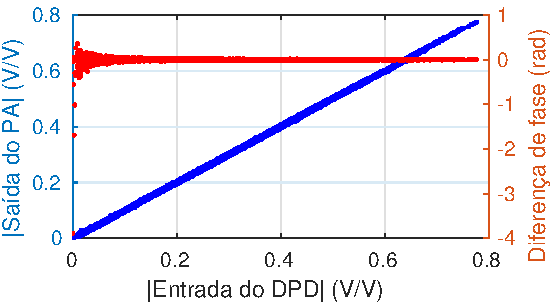
\includegraphics[scale=0.9]{fig2/fig_dpd_ldmos.pdf}
\label{fig:bf-dpd_ldmos}
}\\
\subfloat[GaN{\_}AB{\_}1]{
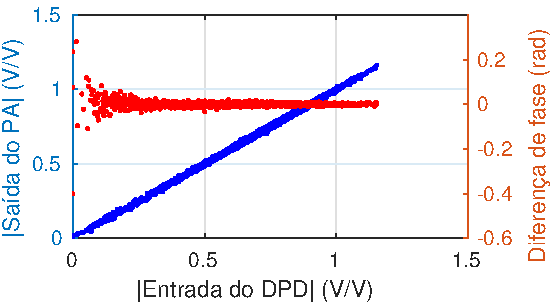
\includegraphics[scale=0.9]{fig2/fig_dpd_sbrt2.pdf}
\label{fig:bf-dpd_sbrt2}
}\\
\subfloat[GaN{\_}AB{\_}2]{
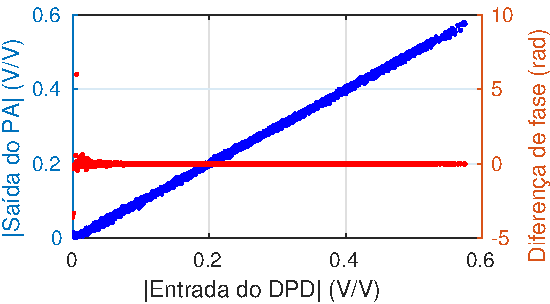
\includegraphics[scale=0.9]{fig2/fig_dpd_tc.pdf}
\label{fig:bf-dpd_tc}
}\\
\subfloat[GaN{\_}Doherty]{
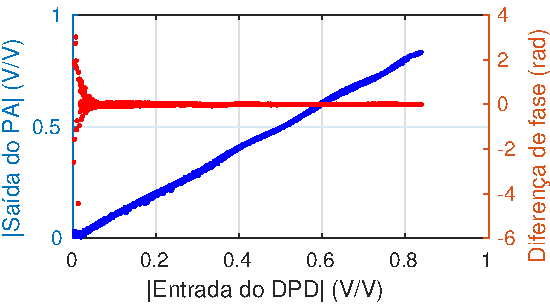
\includegraphics[scale=0.9]{fig2/fig_dpd_doherty.pdf}
\label{fig:bf-dpd_doherty}
}
\caption{Amplitude de saída do PA e diferença de fase na cascata em função da amplitude de entrada do DPD para os diferentes PAs.}
\label{fig:bf-dpd}
\end{figure}


\begin{figure}[H]
\centering
\subfloat[LDMOS{\_}AB]{
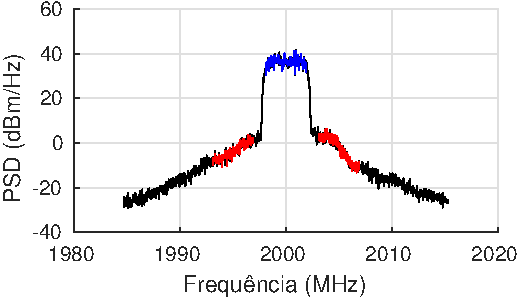
\includegraphics[scale=0.9]{fig2/Frequencia_extraction_ldmos.pdf}
\label{fig:bf-psd_ldmos}
}\\
\subfloat[GaN{\_}AB{\_}1]{
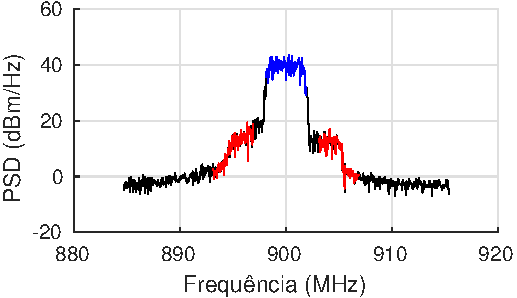
\includegraphics[scale=0.9]{fig2/Frequencia_extraction_sbrt2.pdf}
\label{fig:bf-psd_sbrt2}
}\\
\subfloat[GaN{\_}AB{\_}2]{
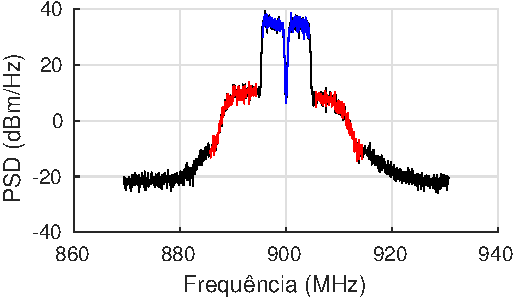
\includegraphics[scale=0.9]{fig2/Frequencia_extraction_tc.pdf}
\label{fig:bf-psd_tc}
}\\
\subfloat[GaN{\_}Doherty]{
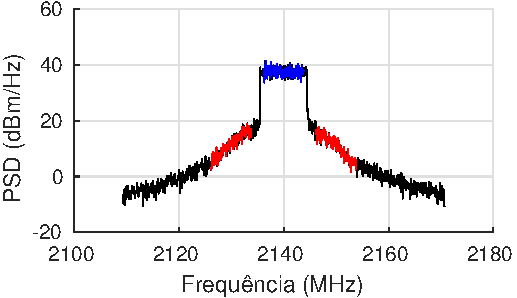
\includegraphics[scale=0.9]{fig2/Frequencia_extraction_doherty.pdf}
\label{fig:bf-psd_doherty}
}\\
\caption{PSD para as entradas estimadas dos DPDs e as saídas medidas dos PAs, considerando-se os conjuntos de dados de treinamento.}
\label{fig:bf-psd}
\end{figure}

